% БҮЛЭГ 6 — ҮР ДҮН БА ХЭЛЭЛЦҮҮЛЭГ

\chapter{Үр дүн ба хэлэлцүүлэг}
\label{Chapter6}

%-------------------------------------------------------------------------------
\section{Хоёр шатлалт нэгдсэн дамжлагын үр дүн}
\label{sec:two-stage-pipeline-results}
\label{sec:e2e}

Энэ хэсэгт хоёр шатлалт MN-BERT нэгдсэн дамжлагын эцсийн дөрвөн ангиллын
гаралтыг үнэлэв. Дамжлагын эхний хэсэг сэтгэгдлийг эерэг, саармаг, сөрөг гэсэн
ерөнхий ангилалд шийднэ. Хэрэв гаралт эерэг эсвэл саармаг бол тухайн шийдвэр
шууд эцсийн ангилал болно. Харин сөрөг гэж шийдэгдсэн сэтгэгдэл хоёрдугаар
шатны MN-BERT ангилагч руу дамжиж, хортой сөрөг эсвэл бүтээлч шүүмжлэл гэсэн
эцсийн хоёр ангиллын аль нэгээр тодорхойлогдоно.

Иймээс энэ хэсэгт дамжлагын эцсийн гаралтаар хэмжигдсэн системийн түвшний
нарийвчлал болон макро-F1 үзүүлэлтийг тайлагнав.

\begin{table}[H]
\centering
\caption{Хоёр шатлалт нэгдсэн дамжлагын системийн түвшний гүйцэтгэл}
\label{tab:two-stage-system}
\fittable{%
\begin{tabular}{@{}p{4.3cm}ccp{4.4cm}@{}}
\toprule
\textbf{Дамжлага} & \textbf{Нарийвчлал} & \textbf{Макро-F1} & \textbf{Тайлбар} \\
\midrule
Хоёр шатлалт MN-BERT нэгдсэн дамжлага & $0.7894$ & $0.7628$ &
Эцсийн дөрвөн ангиллын гаралтаар тооцсон системийн үр дүн \\
\bottomrule
\end{tabular}}
\end{table}

\begin{figure}[H]
\centering
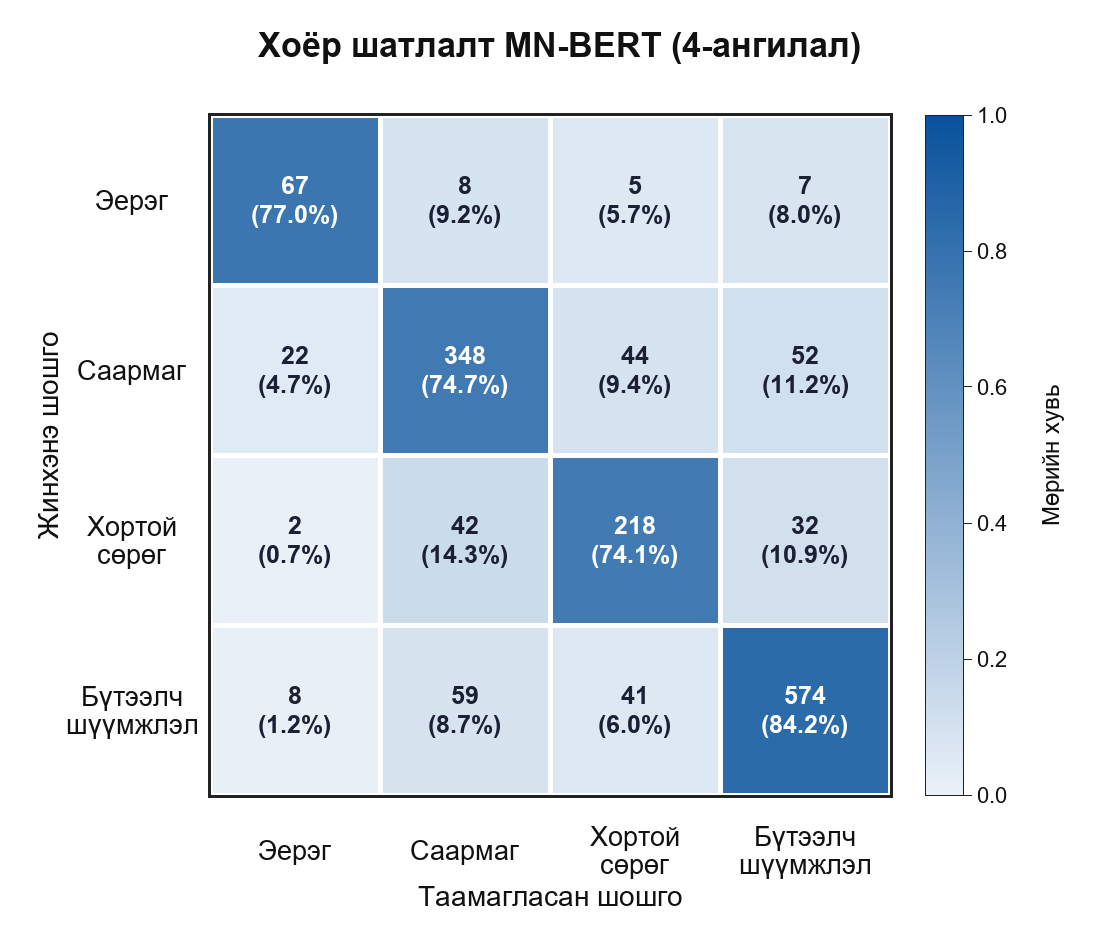
\includegraphics[width=0.75\textwidth]{Figures/CM/cm_two_stage.png}
\caption{Хоёр шатлалт нэгдсэн дамжлагын эцсийн гаралтын төөрөлдлийн матриц}
\label{fig:two-stage-confusion-visual}
\end{figure}

\begin{figure}[H]
\centering
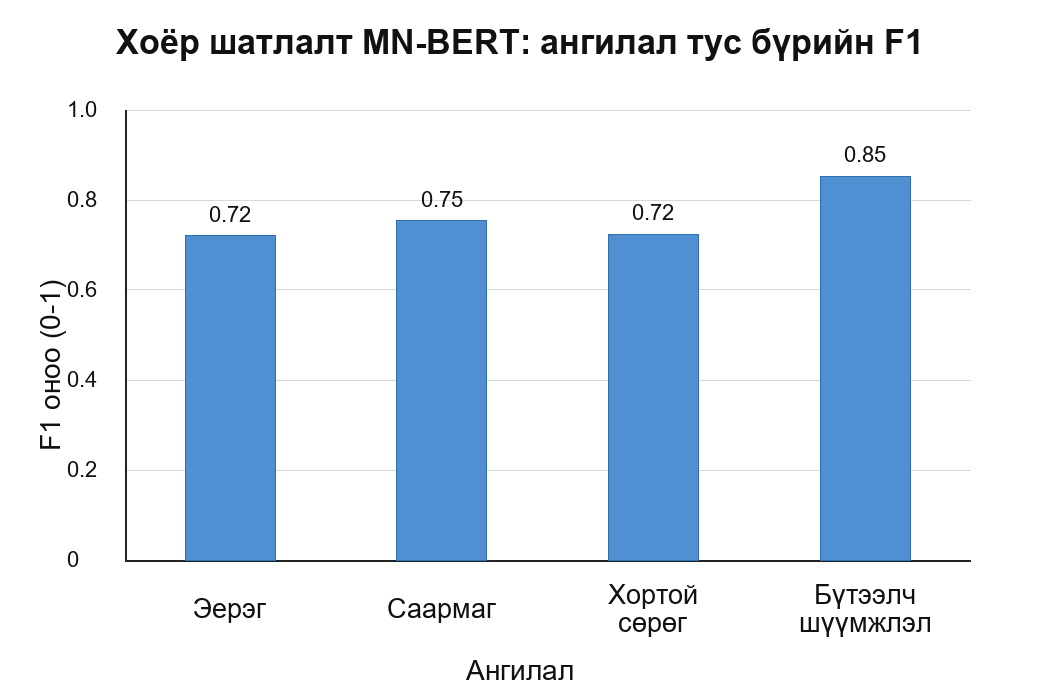
\includegraphics[width=0.75\textwidth]{Figures/CM/two_stage_f1_bar.png}
\caption{Хоёр шатлалт нэгдсэн дамжлагын эцсийн гаралтаас тооцсон ангилал тус бүрийн F1 оноо}
\label{fig:two-stage-f1-bar}
\end{figure}

Зураг~\ref{fig:two-stage-confusion-visual}-д уг төөрөлдлийн матрицыг мөрийн
хувиар дүрслэн харуулж, Зураг~\ref{fig:two-stage-f1-bar}-д ангилал тус бүрийн
F1 оноог нэгтгэн үзүүлэв.

\medskip
\noindent\textbf{Шат дамжсан алдаа ба хоёр шатлалт зохион байгуулалтын хязгаарлалт.}\par

Хоёр шатлалт дамжлагын туршилтын үр дүнгээс харахад \textbf{шат дамжсан алдаа},
өөрөөр хэлбэл эхний шатны буруу шийдвэр дараагийн шатанд дамжин эцсийн ангиллын
үр дүнд нөлөөлөх үзэгдэл нь энэ зохион байгуулалтын гол хязгаарлалтын нэг болж
байна. Эхний шийдвэрлэх хэсэг текстийг эерэг / саармаг / сөрөг гэж ялгахдаа
нийт $1{,}529$ туршилтын дээжээс дараах алдаануудыг гаргасан:

\begin{itemize}
    \item \textbf{Хуурамч сөрөг (87 дээж):} Бодитоор хортой сөрөг эсвэл бүтээлч шүүмжлэл
    байсан 87 сэтгэгдлийг эхний шийдвэрлэх хэсэг ``саармаг'' эсвэл ``эерэг'' гэж
    буруу ангилсан. Үүний үр дүнд эдгээр дээжүүд хоёрдугаар шатанд хүрч чадалгүй,
    эцсийн нарийвчилсан ангилалд буруу туссан.
    \item \textbf{Хуурамч эерэг (145 дээж):} Бодитоор эерэг эсвэл саармаг
    байсан 145 сэтгэгдлийг эхний шийдвэрлэх хэсэг ``Сөрөг'' гэж буруу ангилж,
    хоёрдугаар шат руу дамжуулсан. Энэ нь хоёрдугаар шатны ачааллыг нэмэгдүүлж, эцсийн
    ангиллын нарийвчлалыг бууруулсан.
\end{itemize}

Шат дамжсан алдааны нөлөөгөөр системийн нэгдсэн нарийвчлал $78.94\%$, макро-F1
$0.7628$ болсон нь нэг шатлалт загварын гүйцэтгэлээс ($83.26\%$, макро-F1
$0.8062$) доогуур үзүүлэлт юм. Иймд нэг шатлалт загварыг эцсийн шийдэл болгон
сонгосон.

\medskip
\noindent\textbf{Хоёр шатлалт шийдвэрлэлтийн дүрмийн туршилт.}\par

Шат дамжсан алдааны нөлөөг бууруулах боломжийг шалгахын тулд хоёр шатлалт
хувилбарын хадгалсан гаралтын магадлалыг ашиглан хэд хэдэн шийдвэрлэлтийн дүрэм
туршив. Үүнд нэгдүгээр шатнаас хоёрдугаар шат руу дамжуулах босго утгыг өөрчлөх
болон хоёр шатны магадлалыг хамтад нь ашигласан хөнгөн логистик регрессийн
шийдвэрлэгч загвар багтсан. Энэ нь Хүснэгт~\ref{tab:two-stage-system}-д үзүүлсэн үндсэн
нэгдсэн үнэлгээг орлох бус, хадгалсан гаралтаар шийдвэрлэлтийн дүрэм өөрчлөхөд
ямар нөлөө гарахыг шалгасан нэмэлт туршилт юм.

\begin{table}[H]
\centering
\caption{Хоёр шатлалт шийдвэрлэлтийн дүрмийн хувилбаруудын үр дүн}
\label{tab:two-stage-rules}
\fittable{%
\begin{tabular}{@{}lcc@{}}
\toprule
\textbf{Хувилбар} & \textbf{Нарийвчлал} & \textbf{Макро-F1} \\
\midrule
Үндсэн хоёр шатлалт шийдвэр & $0.7894$ & $0.7628$ \\
Зөөлрүүлсэн хоёр шатлалт шийдвэр & $0.7894$ & $0.7628$ \\
Хатуу босготой шийдвэр & $0.7914$ & $0.7656$ \\
\textbf{Хөнгөн логистик регрессийн шийдвэрлэгч загвар} & $\mathbf{0.7920}$ & $\mathbf{0.7683}$ \\
\bottomrule
\end{tabular}}
\end{table}

\noindent\textit{Тэмдэглэл:} ``Үндсэн хоёр шатлалт шийдвэр'' мөр нь
Хүснэгт~\ref{tab:two-stage-system}-ийн нэгдсэн дамжлагын үр дүнтэй ижил бөгөөд
бусад мөрүүд нь хадгалсан гаралтын магадлалаар шийдвэрлэлтийн дүрэм өөрчлөхөд
гарах нөлөөг харуулна.\par

Үр дүнгээс харахад дамжуулах босго утгыг зөөлрүүлсэн хувилбар нь үндсэн хоёр шатлалт
хувилбараас ялгараагүй. Харин босго нөхцөлийг илүү хатуу тохируулах болон
хоёр шатны магадлалыг хамтад нь ашигласан хөнгөн логистик регрессийн шийдвэрлэгч загвар
бага хэмжээний сайжрал үзүүлсэн. Энэ шийдвэрийн дүрмийн туршилтад хамгийн өндөр
макро-F1 $0.7683$ байв.

%-------------------------------------------------------------------------------
\section{Нэг шатлалт MN-BERT загварын үр дүн}
\label{sec:one-stage-results}

\noindent\textbf{Ангилал тус бүрийн гүйцэтгэл.}\par

\begin{table}[H]
\centering
\caption{Нэг шатлалт MN-BERT загварын ангилал тус бүрийн гүйцэтгэл}
\label{tab:e2e}
\fittable{%
\begin{tabular}{@{}lcccc@{}}
\toprule
\textbf{Үзүүлэлт} & \textbf{Эерэг} & \textbf{Саармаг} & \textbf{Хортой сөрөг} & \textbf{Бүтээлч шүүмжлэл} \\
\midrule
Таамаглалын нарийвчлал & $0.7253$ & $0.8146$ & $0.8125$ & $0.8666$ \\
Сэргээлт      & $0.7586$ & $0.7918$ & $0.7959$ & $0.8856$ \\
F1 оноо      & $0.7416$ & $0.8030$ & $0.8041$ & $0.8760$ \\
Дээжийн тоо & $87$     & $466$    & $294$    & $682$    \\
\midrule
\multicolumn{5}{l}{\textbf{Нийт макро-F1 оноо (4 ангилал):} $\mathbf{0.8062}$} \\
\multicolumn{5}{l}{\textbf{Нийт нарийвчлал (Accuracy):} $\mathbf{0.8326}$} \\
\bottomrule
\end{tabular}}
\end{table}

\begin{figure}[H]
\centering
\begin{tikzpicture}
\begin{axis}[
  ybar,
  bar width=22pt,
  width=0.78\textwidth,
  height=5.8cm,
  enlarge x limits=0.22,
  xtick={1,2,3,4},
  xticklabels={Эерэг, Саармаг, {Хортой сөрөг}, {\shortstack{Бүтээлч\\шүүмжлэл}}},
  ymin=0, ymax=1.05,
  ytick={0,0.2,0.4,0.6,0.8,1.0},
  ylabel={F1 оноо (0--1)},
  ymajorgrids=true,
  grid style={dashed, gray!25},
  nodes near coords,
  every node near coord/.style={font=\small, anchor=south},
  x tick label style={font=\small},
  y tick label style={font=\small},
]
\addplot[fill=blue!52, draw=blue!72]
  coordinates {(1,0.7416)(2,0.8030)(3,0.8041)(4,0.8760)};
\end{axis}
\end{tikzpicture}
\caption{Эцсийн нэг шатлалт MN-BERT загварын ангилал тус бүрийн F1 оноо}
\label{fig:perclass-f1}
\end{figure}

Фокус алдагдлын функц (Focal Loss) нь цөөнх ангиллын алдаанд илүү өндөр жин өгдөг тул
хортой сөрөг зэрэг харьцангуй цөөн жишээтэй ангиллын ялгалтыг дэмжсэн гэж
үзэж болно. Нэг шатлалт загварын төөрөлдлийн матрицыг
Зураг~\ref{fig:confusion}-д харуулав.

\begin{figure}[H]
\centering
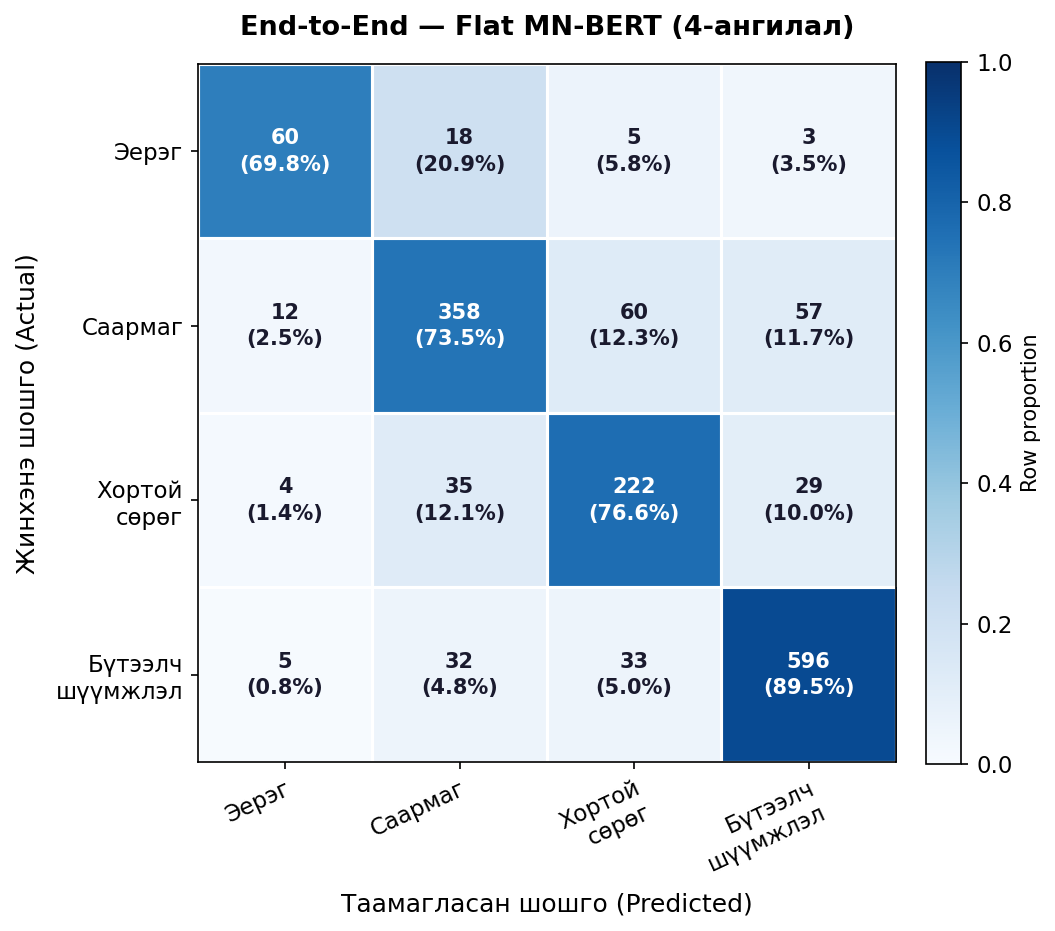
\includegraphics[width=0.75\textwidth]{Figures/CM/cm_e2e.png}
\caption{Нэг шатлалт MN-BERT загварын төөрөлдлийн матриц}
\label{fig:confusion}
\end{figure}

\medskip
\noindent\textbf{Өгөгдлийн чанаржуулалтын нөлөө ба нийт гүйцэтгэл.}\par
\label{sec:label-correction}

Өгөгдлийн багцын чанарыг олон үе шаттай дахин шошгололтоор сайжруулсан
(Хүснэгт~\ref{tab:dq-progression}): нарийвчлал $0.7253\to0.8326$,
макро-F1 $0.7024\to0.8062$ (McNemar $p<0.001$; bootstrap 95\% CI:
нарийвчлал $[0.812,0.851]$, макро-F1 $[0.779,0.829]$).
Шошгололтын үлдэгдэл алдаа бүрэн арилаагүй тул давтан шошгололт хийх нь
цаашдын ажлын нэг чиглэл болно.

Фокус алдагдлын функц (Focal Loss) болон косинус хуваарьтай халаалт (cosine warmup)-ын
тохиргоогоор ($\mathtt{sota\_corrected}$, bs=16, lr=$3{\times}10^{-5}$,
max\_length=256) сургасан нэг шатлалт загварын үр дүнг
Хүснэгт~\ref{tab:corrected-results}-д харуулав.

\begin{table}[H]
\centering
\caption{Нэг шатлалт MN-BERT загварын нэгдсэн үр дүн}
\label{tab:corrected-results}
\fittable{%
\begin{tabular}{@{}p{5.5cm}p{3cm}p{3cm}@{}}
\toprule
\textbf{Загвар} & \textbf{Нарийвчлал (Acc)} & \textbf{Макро-F1} \\
\midrule
Нэг шатлалт MN-BERT (сайжруулсан суурь хувилбар) & $0.8143$ & $0.7760$ \\
\textbf{Нэг шатлалт MN-BERT (эцсийн загвар)} & $\mathbf{0.8326}$ & $\mathbf{0.8062}$ \\
\bottomrule
\end{tabular}}
\end{table}

Өгөгдлийн чанаржуулалтын нөлөөг хэмжихийн тулд загварын хувилбар бүрийн
(ижил MN-BERT архитектур, ижил $1{,}529$ туршилтын олонлог) гүйцэтгэлийг
Хүснэгт~\ref{tab:dq-progression}-д харьцуулав.

\begin{table}[H]
\centering
\caption{Өгөгдлийн чанаржуулалтын явц дахь туршилтын гүйцэтгэл}
\label{tab:dq-progression}
\fittable{%
\begin{tabular}{@{}lp{4.6cm}cc@{}}
\toprule
\textbf{Хувилбар} & \textbf{Өгөгдлийн төлөв} & \textbf{Нарийвчлал} & \textbf{Макро-F1} \\
\midrule
v1 (эхэн)        & анхны шошгололт            & $0.7656$ & $0.7235$ \\
v4               & анхны + өгөгдөл нэмэгдүүлэлт       & $0.7253$ & $0.7024$ \\
v5               & анхны + өгөгдөл нэмэгдүүлэлт       & $0.7456$ & $0.7078$ \\
v6               & дахин шошголсон            & $0.7907$ & $0.7652$ \\
v7               & давхар дахин шошголсон     & $0.8064$ & $0.7698$ \\
Сайжруулсан суурь & v7 (фокус алдагдлын функц + косинус хуваарьтай халаалт) & $0.8143$ & $0.7760$ \\
\textbf{Эцсийн}  & v7 чанаржуулсан хувилбар   & $\mathbf{0.8326}$ & $\mathbf{0.8062}$ \\
\midrule
\multicolumn{2}{@{}l}{\textbf{Нийт сайжралт (v4 $\to$ эцсийн, нэгж):}} & $\mathbf{+10.73}$ & $\mathbf{+10.38}$ \\
\bottomrule
\end{tabular}}
\end{table}

v5$\to$v6 шилжилт дангаараа $+4.5$ нэгжийн сайжралт авчирсан; нийт $+10.73$ нэгж сайжралт статистикийн хувьд ач холбогдолтой (McNemar $p<0.001$).

%-------------------------------------------------------------------------------
\section{Архитектурын хувилбаруудын харьцуулалт}
\label{sec:comparison}

Архитектурын хувилбаруудыг харьцуулахдаа зөвхөн эцсийн гаралтын системийн
түвшний нарийвчлал болон макро-F1 үзүүлэлтийг ашиглав. Харьцуулалтад
суурь загвар, хоёр шатлалт нэгдсэн дамжлага, хуваалцсан энкодертой олон
гаралттай MN-BERT хувилбар болон нэг шатлалт MN-BERT-ийн эцсийн үр дүнг
оруулав.

\begin{table}[H]
\centering
\caption{Архитектурын хувилбаруудын системийн түвшний гүйцэтгэлийн харьцуулалт}
\label{tab:comparison-summary}
\fittable{%
\begin{tabular}{@{}p{4.5cm}ccp{4.1cm}@{}}
\toprule
\textbf{Загвар} & \textbf{Нарийвчлал} & \textbf{Макро-F1} & \textbf{Тайлбар} \\
\midrule
Суурь загвар (SVM, TF-IDF) & $0.6691$ & $0.5733$ & Уламжлалт суурь загвар \\
Хоёр шатлалт MN-BERT нэгдсэн дамжлага & $0.7894$ & $0.7628$ &
Дамжлагын эцсийн дөрвөн ангиллын гаралт \\
Хуваалцсан энкодертой олон гаралттай MN-BERT & $0.8241$ & $0.7972$ &
Нэг энкодер, хоёр ангилагч толгойтой хувилбар \\
\textbf{Нэг шатлалт MN-BERT} & $\mathbf{0.8326}$ & $\mathbf{0.8062}$ &
\textbf{Дөрвөн ангиллыг шууд ялгасан эцсийн загвар} \\
\bottomrule
\end{tabular}}
\end{table}

Хоёр шатлалт хувилбар нь эцсийн нэг шатлалт загварт хэрэглэсэн фокус алдагдлын
функц (Focal Loss) болон косинус хуваарьтай халаалт (cosine warmup)-ын ижил
тохиргоогоор дахин сургагдаагүй. Тиймээс энэ харьцуулалт нь одоо байгаа
нэгдсэн хоёр шатлалт дамжлага ба эцсийн нэг шатлалт загварын системийн
түвшний харьцуулалт бөгөөд бүрэн ижил сургалтын нөхцөлтэй харьцуулахын тулд
хоёр шатлалт хувилбарыг мөн адил тохиргоогоор дахин сургах шаардлагатай.

Хоёр шатлалт зохион байгуулалтын тооцооллын давхардлыг багасгах зорилгоор хоёр
тусдаа MN-BERT энкодер ашигласан үндсэн хувилбараас гадна хуваалцсан
энкодертой (shared encoder) хувилбар туршив. Энэ хувилбарт нэг MN-BERT
энкодерийн гаралтад ерөнхий ангиллын толгой болон сөрөг ангиллын дотоод
ялгалтын толгойг тус тус холбосон.

Үр дүнд нь үндсэн хоёр шатлалт нэгдсэн дамжлагын $0.7894$ нарийвчлал, $0.7628$
макро-F1 нь $0.8241$ нарийвчлал, $0.7972$ макро-F1 болж, нарийвчлал $+0.0347$,
макро-F1 $+0.0345$-аар сайжирсан. Гэсэн хэдий ч энэ хувилбар нь нэг шатлалт
MN-BERT загварын $0.8326$ нарийвчлал, $0.8062$ макро-F1 үзүүлэлтэд хүрээгүй.

\begin{figure}[H]
\centering
\begin{tikzpicture}
\begin{axis}[
  ybar,
  bar width=10pt,
  width=0.82\textwidth,
  height=6.2cm,
  enlarge x limits=0.35,
  symbolic x coords={Separate, Shared},
  xticklabels={{\shortstack{Тусдаа\\энкодер}}, {\shortstack{Хуваалцсан\\энкодер}}},
  xtick=data,
  ymin=0.70, ymax=0.90,
  ytick={0.70,0.75,0.80,0.85,0.90},
  ylabel={Үзүүлэлт (0--1)},
  ymajorgrids=true,
  grid style={dashed, gray!25},
  x tick label style={font=\small},
  y tick label style={font=\small},
  legend style={at={(0.5,-0.20)}, anchor=north, legend columns=2, font=\small},
]
\addplot[fill=orange!62, draw=orange!82, bar shift=-8pt]
  coordinates {(Separate,0.7894)(Shared,0.8241)};
\addplot[fill=blue!52, draw=blue!72, bar shift=8pt]
  coordinates {(Separate,0.7628)(Shared,0.7972)};
\legend{Нарийвчлал, Макро-F1}
\end{axis}
\end{tikzpicture}
\vspace{0.60cm}
\caption{Тусдаа болон хуваалцсан энкодертой хоёр шатлалт хувилбаруудын системийн түвшний харьцуулалт}
\label{fig:two-stage-encoder-sharing-bar}
\end{figure}

\begin{figure}[H]
\centering
\begin{tikzpicture}
\begin{axis}[
  ybar,
  bar width=8pt,
  width=0.92\textwidth,
  height=6.4cm,
  enlarge x limits=0.18,
  symbolic x coords={Base, TwoStage, Shared, OneStage},
  xticklabels={{\shortstack{Суурь\\SVM}}, {\shortstack{Хоёр шатлалт\\MN-BERT}},
    {\shortstack{Хуваалцсан\\энкодер}}, {\shortstack{Нэг шатлалт\\MN-BERT}}},
  xtick=data,
  ymin=0, ymax=1.05,
  ytick={0,0.2,0.4,0.6,0.8,1.0},
  ylabel={Үзүүлэлт (0--1)},
  ymajorgrids=true,
  grid style={dashed, gray!25},
  x tick label style={font=\small},
  y tick label style={font=\small},
  legend style={at={(0.5,-0.26)}, anchor=north, legend columns=2, font=\small},
]
\addplot[fill=orange!62, draw=orange!82, bar shift=-7pt]
  coordinates {(Base,0.6691)(TwoStage,0.7894)(Shared,0.8241)(OneStage,0.8326)};
\addplot[fill=blue!52, draw=blue!72, bar shift=7pt]
  coordinates {(Base,0.5733)(TwoStage,0.7628)(Shared,0.7972)(OneStage,0.8062)};
\legend{Нарийвчлал, Макро-F1}
\end{axis}
\end{tikzpicture}
\vspace{0.85cm}
\caption{Архитектурын хувилбаруудын системийн түвшний гүйцэтгэлийн харьцуулалт}
\label{fig:comparison-bar}
\end{figure}

MN-BERT нь суурь загваруудаас давуу гарсан гол шалтгаан: дэд үгийн токенчлол нь
залгамал бүтцийг ерөнхийлж, анхаарлын механизм нь давхар утга, үгүйсгэлийг
таньдаг, Монгол хэл дээрх урьдчилсан сургалт нь нарийн тохируулгын чанартай
суурь болдог.

Нэг шатлалт эцсийн загварыг суурь, хоёр шатлалт нэгдсэн дамжлага, хуваалцсан
энкодертой хувилбар болон өмнөх MN-BERT ажилтай харьцуулсан үр дүнг
Хүснэгт~\ref{tab:final-scoreboard}-д харуулав.

\begin{table}[H]
\centering
\caption{Эцсийн үр дүнгүүдийн харьцуулалт}
\label{tab:final-scoreboard}
\fittable{%
\begin{tabular}{@{}p{5.5cm}ccp{4.0cm}@{}}
\toprule
\textbf{Загвар} & \textbf{Нарийвчлал} & \textbf{Макро-F1} & \textbf{Тайлбар} \\
\midrule
Суурь загвар (SVM, TF-IDF) & $0.6691$ & $0.5733$ & Уламжлалт суурь \\
Хоёр шатлалт MN-BERT нэгдсэн дамжлага & $0.7894$ & $0.7628$ & Дамжлагын эцсийн гаралт \\
Хуваалцсан энкодертой олон гаралттай MN-BERT & $0.8241$ & $0.7972$ & Нэг энкодер + хоёр ангилагч толгой \\
Нэг шатлалт MN-BERT (сайжруулсан суурь хувилбар) & $0.8143$ & $0.7760$ & Анхны сайжруулсан хувилбар \\
\textbf{Нэг шатлалт MN-BERT (эцсийн загвар)}   & $\mathbf{0.8326}$ & $\mathbf{0.8062}$ & Фокус алдагдлын функц + косинус хуваарьтай халаалт \\
\midrule
Өмнөх диплом 1 (MN-BERT нарийн тохируулга) & $0.8270$ & $0.8100$ & 3 ангилалт хандлагын ангилал \\
\bottomrule
\end{tabular}}
\end{table}

Эцсийн загвар ($0.8326$) нь өмнөх диплом 1-ийн хандлагын ангилагчийн
нарийвчлалаас ($0.8270$) бага хэмжээгээр давсан. Гэхдээ тухайн ажил нь өөр
ангиллын тогтолцоотой тул энэ мөрийг зөвхөн Монгол хэл дээр MN-BERT нарийн
тохируулсан өмнөх ажлын ерөнхий лавлах түвшинд авч үзэв.

%-------------------------------------------------------------------------------
\section{Алдааны дүн шинжилгээ}
\label{sec:error-analysis}

Нэг шатлалт MN-BERT загварын туршилтын өгөгдөл дээрх нийт $256$ буруу ангилагдсан дээжийг гараар шалгаж
гурван давамгайлах хэв маягийг тодорхойлов.
Доорх жишээнүүд нь \texttt{test\_predictions\_sota\_corrected.csv} файлаас
сонгосон \textbf{бодит буруу ангилагдсан} дээжүүд юм.

\textbf{Жишээ 1 — Бүтээлч шүүмжлэл $\to$ Хортой сөрөг (id=5104):}
\begin{quote}
``Авилгалын загалмайлсан эцэг бага донгосоорой. Чиний улсад учруулсан
хохирол бага биш шүү. Нэмж хорлохоо болиорой.''
\end{quote}
Жинхэнэ ангилал: \textit{бүтээлч шүүмжлэл}. Таамагласан: \textit{хортой сөрөг}.
\emph{Шалтгаан:} ``Авилгалын загалмайлсан эцэг'' гэх нэрлэлт нь хувийн
халдлагын лексик жинтэй бөгөөд загвар эдгээр лексик шинжид илүү тулгуурласан
байж болзошгүй.
Гэвч ``Нэмж хорлохоо болиорой'' гэх тушаалт хэлбэр нь зан үйлийн тодорхой
өөрчлөлт шаарддаг --- энэ нь бүтээлч шүүмжлэлийн гол шинж юм.
MN-BERT нэрлэлтийн лексик жинг тушаалт бүтцийн зорилгод давамгайлуулж байна.

\textbf{Жишээ 2 — Хортой сөрөг $\to$ Бүтээлч шүүмжлэл (id=4436):}
\begin{quote}
``Оюу Толгой мөлжлөгөө зогсоо, ард түмний баялгийг дээрэмдэн ачаад бас
манай өр зээлд өндөр хүү тавьсан мөлжлөг. Үгүй бол уурхайн амуудыг
пуужин ба дроноор нураана.''
\end{quote}
Жинхэнэ ангилал: \textit{хортой сөрөг}. Таамагласан: \textit{бүтээлч шүүмжлэл}.
\emph{Шалтгаан:} Эхний өгүүлбэр ``мөлжлөгөө зогсоо'', ``ард түмний баялгийг''
гэх хэлбэрээр байгууллага, эдийн засгийн үйл ажиллагаанд чиглэсэн шүүмжлэлийн
зарим шинжийг агуулдаг.
Загвар энэ эхний агуулгад суурилж бүтээлч шүүмжлэл гэж ангилсан.
Харин ``пуужин ба дроноор нураана'' гэх хүчирхийллийн заналхийлэл сүүлийн
өгүүлбэрт нэмэгдэж байгааг загвар дутуу тусгасан --- өгүүлбэр доторх
зорилгын хурдан хувьсал анхаарлын механизмд хангалттай мэдрэгддэггүй.

\textbf{Жишээ 3 — Саармаг $\to$ Бүтээлч шүүмжлэл (id=219):}
\begin{quote}
``Ийм шийдвэрт Ерөнхийлөгч хориг тавих нь УИХ-ын бүрэн эрхэд
халдсан гэж үздэг.''
\end{quote}
Жинхэнэ ангилал: \textit{саармаг}. Таамагласан: \textit{бүтээлч шүүмжлэл}.
\emph{Шалтгаан:} ``УИХ-ын бүрэн эрхэд халдсан'' гэх агуулгын үгс нь улс
төрийн шүүмжлэлтэй хэлбэрийн хувьд ижил; загвар энд татагдсан.
Гэвч ``гэж үздэг'' гэх хэлц нь Монгол хэлний эвидентиаль тэмдэглэгч
(evidential marker) буюу бусдын байр суурийг мэдэгдэж байгаа саармаг
тайлбар юм. `Гэж үздэг', `гэсэн', `гэх мэт' зэрэг эвидентиаль бүтэц нь
сургалтын хуваарилалтад дутуу төлөөлдөг тул загварт саармагжуулах
дохио болж ажилладаггүй.

Гол хязгаарлалт: (1)~лексик нэрлэлтийн жин ба тушаалт бүтцийн зорилго,
(2)~эхний өгүүлбэрийн бүтээлч давамгайлал ба сүүлийн хэсгийн хүчирхийллийн
даамжрал, (3)~Монгол хэлний эвидентиаль тэмдэглэгч загварт мэдрэгдэхгүй байх
(цаашдын чиглэл: бүлэг~\ref{Chapter8}).

%-------------------------------------------------------------------------------
\section{Таамаглалын баталгаажилт}
\label{sec:hypothesis-check}

Бүлэг~\ref{Chapter1}-д дэвшүүлсэн дэд таамаглалуудыг туршилтын үр дүнтэй
харьцуулан дүгнэв:

\begin{itemize}
  \item \textbf{H$_1$ (батлагдсан):} Хортой сөрөг агуулга ба бүтээлч
    шүүмжлэлийг тусдаа ангиллаар авч үзэх нь андуурлын хэв шинжийг илүү
    тодорхой харуулсан. Эцсийн нэг шатлалт загвар нийт $83.26\%$ нарийвчлал,
    $\mathbf{0.8062}$ макро-F1 үзүүлсэн боловч ангилал тус бүрийн F1 оноо
    ялгаатай гарсан: хортой сөрөг ангилалд $0.8041$, бүтээлч шүүмжлэл
    ангилалд $0.8760$ (Хүснэгт~\ref{tab:e2e}). Иймээс эдгээрийг нэг
    ``сөрөг'' ангилалд нэгтгэн тайлагнавал хоёр ангиллын хооронд үүсэх
    андуурлын хэв шинж харагдахгүй үлдэх байв.
  \item \textbf{H$_2$ (батлагдсан):} Өгөгдлийн чанаржуулалтын нөлөөгөөр
    нарийвчлал $0.7253\to0.8326$, макро-F1 $0.7024\to0.8062$ болж өссөн
    (Хүснэгт~\ref{tab:dq-progression}, McNemar $p<0.001$). Энэ нь маргаантай
    жишээг дахин нягтлах, давхардал болон шошгололтын зөрчлийг багасгах зэрэг
    алхам нь загварын эцсийн гүйцэтгэлд бодит нөлөө үзүүлснийг харуулна.
  \item \textbf{H$_3$ (батлагдсан):} Хоёр шатлалт зохион байгуулалт нь сөрөг
    ангиллыг хортой сөрөг ба бүтээлч шүүмжлэл болгон нарийвчлах тайлбарлагдахуйц
    бүтэцтэй боловч шат дамжсан алдааны нөлөө бодитоор илэрсэн. Нэгдсэн
    хоёр шатлалт дамжлагын нийт системийн гүйцэтгэл $78.94\%$ нарийвчлал,
    $0.7628$ макро-F1 болж, нэг шатлалт загварын $83.26\%$ нарийвчлал,
    $0.8062$ макро-F1 үзүүлэлтээс доогуур гарсан. Хуваалцсан энкодертой
    олон гаралттай хувилбар $0.8241$ нарийвчлал, $0.7972$ макро-F1 болж
    сайжирсан боловч эцсийн нэг шатлалт загварт хүрээгүй.
    Иймээс нэг шатлалт загварыг эцсийн шийдэл болгон сонгох үндэслэл болов.
\end{itemize}

%-------------------------------------------------------------------------------
\section{Бүлгийн дүгнэлт}

Энэ бүлэгт хоёр шатлалт нэгдсэн дамжлага, хуваалцсан энкодертой олон гаралттай
MN-BERT, нэг шатлалт MN-BERT болон TF-IDF суурь загваруудын үр дүнг системийн
түвшинд харьцуулан хэлэлцэв. Хоёр шатлалт зохион байгуулалт нь эцсийн гаралтын
түвшинд шат дамжсан алдаанд мэдрэмтгий байж, нэг шатлалт MN-BERT загвараас
доогуур гүйцэтгэлтэй гарсан. Хуваалцсан энкодертой хувилбар энэ үзүүлэлтийг
$0.8241$ нарийвчлал, $0.7972$ макро-F1 хүртэл сайжруулсан ч нэг шатлалт эцсийн
загвараас доогуур байв. Чанаржуулсан өгөгдөл болон фокус алдагдлын функц,
косинус хуваарьтай тохиргоо ашигласан нэг шатлалт MN-BERT нь
$\mathbf{83.26\%}$ нарийвчлал, $\mathbf{0.8062}$ макро-F1 үзүүлсэн тул эцсийн
шийдлээр сонгогдов.
Цаашдын сайжруулалтын чиглэлүүдийг бүлэг~\ref{Chapter8}-д авч үзнэ.
